\section{Measurement choices and historical forecast evaluation}
\subsection{The scoring contract}
For claim $i$, let $m_i$ denote its publication month, $h_i$ its assigned horizon, $q_i$ its target, and $d_i$ its normalized direction. A scoring specification $s$ maps the target and dates to an outcome $y_i^{(s)}$. Correctness is
\begin{equation}
 z_i^{(s)}=\mathbf{1}\{d_i=y_i^{(s)}\}.
 \label{eq:correct}
\end{equation}
This is a definition of correspondence under an interpretation, not a direct measurement of whether the historical speaker understood the economy. If $q_i$ or $h_i$ misrepresents the passage, $z_i^{(s)}$ can be computed exactly and still answer the wrong substantive question.

The inherited outcome rule compares the publication-month level with the level $h_i$ months later. For production, prices, and markets, the change is $100(X_{m_i+h_i}/X_{m_i}-1)$; for unemployment it is the difference in rate percentage points. The original flat bands are $\pm2\%$ for industrial production, $\pm5\%$ for the nominal Shiller S\&P Composite price series, $\pm1.5\%$ for CPI, and $\pm0.5$ percentage points for unemployment. Changes exactly at a boundary count as flat, subject to the saved numerical tolerance.\evidence{H2}

The core outcome series distributed through FRED are industrial production (INDPRO; \citealp{fredindpro}), the consumer price index (CPIAUCNS; \citealp{fredcpi}), and unemployment (UNRATE; \citealp{fredunrate}). The market outcome uses the Shiller stock-price series \citep{shiller}. Payroll employment (PAYEMS) supplies the alternative employment target \citep{fredpayems}. Recession-state coding draws on USREC and the NBER chronology \citep{fredusrec,nber}; these retrospective labels are outcomes or descriptive classifications, not contemporaneously known forecast features. The saved reference files and their hashes identify the numerical vintages actually used. Bibliographic access dates do not identify or update those frozen snapshots.

The price direction uses the explicit price field. Employment uses the explicit unemployment-direction field when available, otherwise mapping improved employment conditions to falling unemployment. This fallback is operationally convenient but not a semantic equivalence. For business and market claims, improve and worsen map to rising and falling benchmark levels. Shiller prices exclude dividends and are a proxy for broad market statements, not an exact benchmark for every asset forecast. Pre-1919 business claims lack industrial-production endpoints and receive a separate NBER-state proxy in the legacy description; they are excluded from the main sensitivity and claim-model samples.

Positive integer horizons from one to twenty-four months are respected. Vague horizons receive six or twenty-four months when the export records a short or long inference, otherwise twelve months. Invalid numeric horizons and unusable labels are excluded rather than clipped. The verified inventory has 142,810 default-horizon claims, underscoring how frequently source timing is not explicit. Moreover, the scorer's ``stated'' category denotes a numeric machine horizon; it does not guarantee that a human recovered that endpoint from the source.

Within a target-specific sample, article-equal accuracy is
\begin{equation}
 \widehat A_s=\frac{1}{J}\sum_{j=1}^{J}\frac{1}{n_j}
     \sum_{i\in j}z_i^{(s)},\qquad
 \widehat\Delta_s=\frac{1}{J}\sum_{j=1}^{J}\frac{1}{n_j}
     \sum_{i\in j}\left[z_i^{(s)}-\mathbf{1}\{b_i=y_i^{(s)}\}\right],
 \label{eq:paired}
\end{equation}
where $n_j$ counts eligible claims in article $j$, $J$ counts articles, and $b_i$ is the comparison forecast. Both forecasts face identical observations, outcomes, and weights. Equal article weighting limits the influence of articles containing many extracted claims; it does not remove common-month economic dependence.

\subsection{The legacy description and raw sensitivity}
On 175,855 scored historical candidates, claim-weighted correctness is 40.8\%, compared with 53.6\% for the fixed-direction rule that predicts rising production, prices, and stock prices and falling unemployment. The baseline is a target-specific directional comparator, not an optimized universal forecast and not a claim that rising prices improve welfare. Under equal article weights, the rates are 40.9\% and 53.6\%, a gap of $-12.7$ percentage points.\evidence{H2}

The raw sensitivity set, processed under the same deterministic rules but on its own eligible support, has article-weighted accuracy 41.7\% against 55.2\% for the baseline. Its gap is $-13.5$ points. Because verification changes composition, the difference between raw and verified rates is not a causal estimate of the verifier's effect on forecast quality. It does show that replacing the primary candidate set with raw exports does not reverse the negative aggregate comparison in this saved exercise.

These pooled results mix targets, eras, horizons, and benchmark availability. They should not be presented as a single universal historical ``accuracy of newspapers.'' The matched employment exercise below deliberately holds the claims and weights fixed to isolate changes in the outcome definition.

\subsection{Changing the flat band on identical employment claims}
The principal sensitivity cohort contains 9,260 verified employment claims from 7,463 articles with numeric machine horizons and non-NBER benchmark support. It compares three recorded specifications: the original half-percentage-point unemployment band, that band multiplied by $h_i/12$, and a zero-width sign-only band. Duration scaling is a linear sensitivity scenario, not a human-validated correction. Sign-only scoring counts even economically tiny nonzero changes. All three use the same claims and article weights.\evidence{M1}

\begin{table}[t]
\caption{Employment scoring sensitivity on common support}\label{tab:employment}
\centering\small
\begin{tabularx}{\linewidth}{Xrrrr}
\toprule
Scoring rule & Claims correct & Baseline & Gap (pp) & 95\% block interval\\
\midrule
Original & 34.2\% & 20.1\% & +14.2 & [3.5, 25.9]\\
Duration scaled & 43.2\% & 27.2\% & +16.0 & [2.3, 30.0]\\
Sign only & 57.6\% & 46.8\% & +10.8 & [$-7.0$, 26.5]\\
\bottomrule
\end{tabularx}
\note{9,260 identical claims, 7,463 articles. The comparator always predicts improvement, operationalized as falling unemployment. Equal total weight per article within this cohort. Intervals are paired five-year calendar-block bootstrap intervals for the gap: 14 occupied blocks and 5,000 draws, conditional on saved scoring choices. They omit interpretation and specification-selection uncertainty. Source: M1.}
\end{table}

\begin{figure}[t]
\centering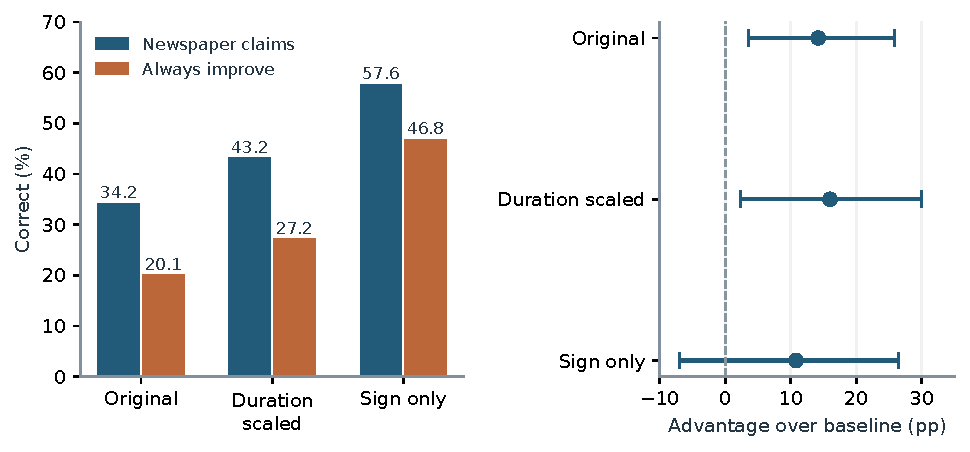
\includegraphics[width=\linewidth]{employment_sensitivity.pdf}
\caption{Higher measured accuracy does not imply a larger advantage over the comparator. Left: claim and baseline correctness under each rule. Right: paired baseline-relative differences with the saved 95\% five-year block intervals. Claims and weights are fixed across specifications.}\label{fig:employment}
\end{figure}

The accuracy increase from 34.2\% to 57.6\% is 23.4 percentage points. Yet the fixed comparator improves by 26.8 points, so the newspaper advantage is smaller under sign-only scoring. The flat-band choice changes which outcomes are common: the always-flat comparator scores 50.6\% under the original rule, 35.2\% under duration scaling, and 5.8\% under sign-only scoring. Under the original band, newspapers underperform always-flat by 16.4 points even though they outperform always-improve. These facts show why reporting only one favorable baseline comparison is incomplete.

The results are descriptive specification sensitivity, not a test that the original band is logically invalid. A tolerance band can be appropriate for a forecast of economically material change. The source might instead commit to any increase, in which case sign-only scoring may be closer. Choosing the rule because it produces the highest hit rate would use outcomes to decide what the forecast meant. Source interpretation should precede that choice.

\subsection{Employment growth and unemployment are different targets}
The alternative-target exercise compares falling unemployment with rising payroll employment on the same 9,260 claims. After orienting both series toward improving labor-market conditions, sign-only outcomes disagree on 21.95\% of article-weighted observations. Employment can grow while the unemployment rate rises, for example if the labor force expands sufficiently. Benchmark disagreement is therefore not automatically a data error. It is evidence that the two economic questions are different.\evidence{M2}

\begin{table}[t]
\caption{Changing the employment benchmark reverses the baseline-relative point estimate}\label{tab:target}
\centering\small
\begin{tabularx}{\linewidth}{Xrrrr}
\toprule
Sign-only outcome & Claims correct & Baseline & Gap (pp) & 95\% block interval\\
\midrule
Unemployment falls & 57.6\% & 46.8\% & +10.8 & [$-7.0$, 26.5]\\
Payroll employment rises & 55.1\% & 63.3\% & $-8.2$ & [$-33.2$, 19.0]\\
\bottomrule
\end{tabularx}
\note{Same 9,260 claims with common endpoint support and equal article weights. Both comparators always predict improving labor-market conditions, mapped to the relevant series. This is an alternative interpretation of broad employment labels, not a source-validated relabeling of every claim. The saved alternative-target exercise also preserves frozen-versus-refreshed-series checks. Source: M2.}
\end{table}

The newspaper hit rate changes only modestly, from 57.6\% to 55.1\%, but the baseline rises from 46.8\% to 63.3\%. The resulting advantage changes by approximately $-19.0$ percentage points. The intervals are wide and include zero for both sign-only comparisons. The robust conclusion is the sensitivity of the point estimates and comparative interpretation, not established newspaper superiority under one target and inferiority under another.

This distinction extends beyond employment. Lower inflation is a decline in the rate of price growth, whereas falling prices are a decline in the price level. Slower output growth can coexist with rising output. A recession onset is an event, whereas an industrial-production endpoint change describes a particular series over a particular interval. An extractor that assigns only a broad topic cannot resolve these meanings by itself.

For fixed claims and weights, an elementary bound clarifies the arithmetic. If the same normalized prediction is scored against two outcome labelings, then
\begin{equation}
 |\widehat A_s-\widehat A_{s'}|
 \leq \frac{\sum_i w_i\mathbf{1}\{y_i^{(s)}\neq y_i^{(s')}\}}{\sum_i w_i}.
 \label{eq:bound}
\end{equation}
Only observations whose outcome labels change can change correctness. This follows directly from the indicator definition and is not offered as a novel theorem. It also does not establish which labeling is right. For a baseline-relative gap, both the claim and comparator terms can change; under the same fixed prediction mapping the analogous bound is twice the weighted disagreement. The empirical task remains identifying the economic proposition in the source.

\subsection{Dependence, uncertainty, and selection}
Claims are not independent economic trials. Multiple articles can discuss the same month, and overlapping horizons share much of the same outcome path. The primary historical sensitivity intervals therefore resample occupied five-year publication blocks in pairs, preserving model or rule comparisons within a block. Two- and ten-year versions are retained in the saved outputs. The employment analysis has 14 occupied five-year blocks; thousands of claims do not create thousands of independent business-cycle realizations.

These intervals condition on the saved observations, interpretations, and fitted outputs. They do not capture uncertainty about source validity, target choice, or the process that selected specifications after earlier results were inspected. The publication specification was written after historical analyses had been viewed. It is not a preregistration, and the sensitivity analyses do not create a fresh holdout. We consequently report their magnitudes and stability rather than promote a winning rule from observed performance.

